\section{Quantisation and Normalisation Group Flow}
\label{sec:Renormalisation}

This section will treat \emph{scalar perturbative quantum field theory}. We will start by giving a general introduction to the matter and then talk about the \emph{Renormalisation group equation}. After introducting \emph{Feynman graphs}, we will finally arrive at the first full definition of a \emph{QFT} and discuss some immediate results. Finally we will discuss the \emph{renormalisation of QFT}.

\subsection{Introduction}
\label{subsec:quantisation_intro}

The main idea of Quantum mechanics is to define a deterministic evolution of a system as a superposition of possible evolutions where one weights them by how likely they are. Our ultimate goal is to describe Quantum mechanics and Classical mechanics in terms of the sets of objects, states and observables. The main idea is to take a state $\omega$ and an observable $A$ such that the state associates a propability distribution to the observable on the real line in the form of $\omega_A(\lambda)$. To illuminate the concepts and systems we aim to unify, we present a short overview of both:\\

In Classical mechanics, states are nothing but normalized measures on the \emph{phase space} (mind: a symplectic manifold). Meanwhile observables are functions on the phase space given by $(p,q)$ such that $\omega = dp \wedge dq$. The propability distribution is then given by
$$ \omega_A (\lambda) := \int_M \theta(\lambda - f_A (p,q)) d \mu_\omega$$
where $\theta$ denotes the step function, $f_A$ an observable and $d\mu_\omega$ a measure corresponding to the state. The dynamics on the other hand are encoded in the \emph{Poisson brackets} defined using the symplectic form $\omega$ as
$$ \dd{f}{t} = \{H, f\} $$
for some functions $H$ which turns out to be the \emph{Hamiltonian} of the system.\\

In Quantum mechanics, observables are linear operators on some complex \emph{Hilbert spae} $\HH$. States are positive trace-class operators with unit trace defined as $\Tr A = \sum_n \langle A e_n, e_n \rangle$. The propability distribution for a state is defined by
$$ \omega_A (\lambda) := \Tr(M P_A(\lambda)) $$
where $M$ is a trace-class (state) and $P_A(\lambda)$ is a projection (observable). Note that we are looking at the field from a mathematical perspective, thus the reader might encounter unfamiliar technical details in this and upcoming discussions.\\
The commutator of two states $A,B$ is defined as
$$ \{A,B\} = \frac{i}{\hbar} (AB-BA) $$
such that the time evolution, given the Hamiltonian operator $H$, is defined as
$$ \dd{A}{t} = \{H,A\} $$
With these classifications of the two fields in mind, we arrive at a first sketch of a transition between them:

\begin{definition}[Quantisation Scheme]
  A map passing from Classical mechanics to Quantum mechanics is called a \textbf{quantisation scheme}.
\end{definition}

To illuminate this rather vague definition, we discuss a "toy example":

\begin{example}[Weyl Quantisation]
  This quantisation treats a mechanical system with one degree of freedom. The classical system has $\RR^2$ as its phase space with coordinates $(p,q)$. The dynamics are given by the Poisson-brackets with the Hamiltonian function. Now we want to transition to a quantum description:\\

  We take the Hilbert-space $\HH$ defined as
  $$ \HH = L^2(\RR) := \left\{ \psi(q) \in C(\RR) \ \Big| \ \int_{-\infty}^\infty |\psi(q)|^2 dq < \infty  \right\} $$
  Observables are now operators on $\HH$. We define the two operators
  $$ (P\psi)(q) = \frac{\hbar}{i} \dd{}{q} \psi(q), \quad \quad (Q\psi)(q) = q \psi(q) $$
  Now we can define products
  $$ (A\psi)(q) = \int_{-\infty}^\infty A(q,q^\prime) \psi(q^\prime) dq^\prime $$
  where $A(q,q^\prime)$ denotes the integral kernel of $A$ defined as
  $$ A(q,q^\prime) = \frac{1}{2 \pi \hbar} \int_{-\infty}^\infty f\left( p, \frac{q+q^\prime}{2} \right) e^{ip(q-q^\prime)/\hbar} dq $$
  where the $f$ are functions that represent $A$ in classical mechanics. As an exercise you can show that with these definitions you obtain the previously defined operators $P,Q$ if you set $f=p$ and $f=q$ respectively.\\

  Next we need to define a product. Since generally $A_{fg} \neq A_f A_g$ we investigate
  $$ A_f A_g (q, q^\prime) = \int_{-\infty}^\infty A_f(q, q^{\prime \prime}) A_g(q^{\prime \prime},q^\prime) dq^{\prime \prime} $$
  and then define
  $$ f *_\hbar g = fg + \frac{i\hbar}{2} \{f,g\} + \mathcal{O}(\hbar^2) \quad \Rightarrow \quad \frac{i}{\hbar} (f *_\hbar g - g *_\hbar f) = \{f,g\} + \mathcal{O}(\hbar^2)$$
  We now encode the dynamics via the time derivative using the Hamiltonian operator
  $$ \dd{A(t)}{t} = \{H, A(t)\}_\hbar , \quad \quad A(0) = A $$
  where we define $A(t)$ as
  $$ A(t) = U^{-1}(t) A U(t), \quad \quad U(t) = e^{-i H t / \hbar} $$
  As an exercise you can prove this in a formal setting. Note that we do not yet have a concrete way to define the exponential of an operator such as $H$. Thus, setting $\hbar = 1$ for simplicity, we investigate the integral kernel of $U = e^{-iH(t^{\prime \prime} - t^\prime)}$ in terms of $h(p,q)$. To this end let $\Delta \ll 1$ such that
  $$ U_\Delta := e^{-i H \Delta} \cong 1- i H \Delta $$
  Thus setting $t^{\prime \prime} - t^\prime = N \Delta$ we obtain $e^{-iH(t^{\prime \prime} - t^\prime)} = (U_\Delta)^N$. Now we calculate
  \begin{align*}
    U_\Delta(q,q^\prime) &= \frac{1}{2\pi} \int_{-\infty}^\infty dp e^{ip(q-q^\prime)} \left( 1- i h\left(p, \frac{q+q^\prime}{2} \right) \Delta \right) \\
    &= \frac{1}{2\pi} \int_{-\infty}^\infty dp e^{ip(q-q^\prime) - i h\left(p, \frac{q+q^\prime}{2} \right) \Delta} + \mathcal{O}(\Delta^2)
  \end{align*}
  Now setting $q = q_N, q^\prime = q_0$ and $q_j$ the $N-1$ intermediate variables, we arrive at the following form:
  \begin{align*}
    U(q, q^\prime, t^{\prime\prime}-t^\prime) &= \int_{-\infty}^\infty ... \int_{-\infty}^\infty \frac{dp_1 dq_1}{2\pi} ... \frac{dp_{N-1} dq_{N-1}}{2\pi} \frac{dp_N}{2\pi}\\
    &\times e^{ip_{N}(q_{N}-q_{N-1}) + ... + ip_1(q_1-q_0)} \cdot e^{-ih\left(p_N, \frac{q_N + q_{N+1}}{2}\right) ... -ih\left( p_1, \frac{q_1 + q_0}{2} \right)}
  \end{align*}

  Thus we take $N\lra \infty$ such that $q_j - q_{j-1}$ being proportional to $\frac{1}{N}$ goes against $0$. While we do not discuss convergence and well-definedness at this point, the reader is invited to start looking critically at these notions from now on! Formally this gives us the following form of $U$ which indeed has many problems with convergence of integrals
  \begin{align*}
    U(q,q^\prime, t^{\prime\prime}-t^\prime) = \int ... \int_{t^\prime}^{t^{\prime\prime}}  \exp\left[i\int_{t^\prime}^{\prime \prime}( p(t)\dot q(t) - h(p(t),q(t)))\ dt \right] \prod_i \frac{dp(t) dq(t)}{2\pi}
  \end{align*}
  Where the first fraction defines our measure on the space of paths from $[t^\prime, t^{\prime\prime}]$ called the \textbf{Liouville-measure} and the term in the exponential is called the \textbf{Action functional}.\\

  Note that this is only a one-dimensional "toy model" which already boasts some pretty severe convergence problems. Since we ultimately aim to define an infinite-dimensional generalisation, the rest of the course will deal with the "taming" of these problems.
\end{example}

In the following we give a short introduction to \textbf{Feynman Path Integrals}, visually respresented in the following picture:
\begin{center}
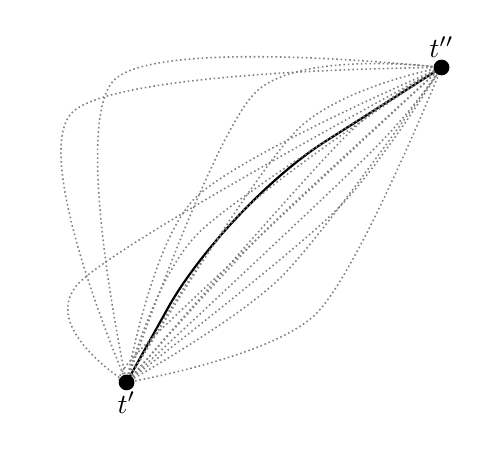
\begin{tikzpicture}[]
\draw[thick, black,rounded corners=15mm] (-2.,-2.) -- (-.75,.25) -- (2,2);

\foreach \j in {1,...,15} {
  \draw[gray,densely dotted, line width = .2mm] plot[smooth] coordinates {(-2.,-2.)(-.75+2*rand,.25+2*rand)(2,2)};
}

\fill [black] (2.,2.) circle (0.1) node[above]{$t^{\prime\prime}$};
\fill [black] (-2.,-2.) circle (0.1) node[below]{$t^\prime$};
\end{tikzpicture}
\end{center}
Feynman's approach to Quantum Field Theory was the idea of a "sum over all possible histories" of a particle. In \emph{chapter 2} \ref{subsec:Classical_field_theory} we already mentioned scalar field theories where $\psi \in\Ci(M)$ is a scalar field. The physical phenomenon corresponding to the "sum over histories" is described by a superposition of all possible scalar theories, weighted by $e^{iS(\psi) / \hbar}$ for $S(\psi)$ the action of $\psi$.\\

This in turn has an interpretation coming from statistical mechanics: Here, $\psi$ would represent the state of a statistical system, $S(\psi)$ would be the systems energy. Given a temperature $T$, the system could be in any state $e^{-S(\psi)/ T}$. Thus we obtain the following correspondence:
\begin{center}
\begin{tikzcd}
  T \arrow[r,leftrightarrow] & i \hbar
\end{tikzcd}
\end{center}
This gives us a sufficient motivation to repeat the assessment of dynamics for statistical systems:\\

In statistical mechanics, observables are maps $O: \Ci(M,\RR) \lra \CC$ and correlation functions between observables are defined as
\begin{align*}
  \langle O_1, ..., O_n \rangle &= \int_\psi e^{-S(\psi)/T} O_1(\psi) ... O_n(\psi) D\psi\\
  \Longrightarrow \quad \quad \langle O_1, ..., O_n \rangle &= \int_{\psi \in \Ci(M)} e^{i S(\psi)/\hbar} O_1(\psi) ... O_n(\psi) D\psi
\end{align*}
The main problem in this situation is that $\Ci(M)$ is an infinite-dimensional vector space.

\begin{rem}~
\begin{itemize}
  \item[(1)] One approach to resolve this is \emph{perturbative QFT} where we work in the limit $\hbar \lra 0$ such that we can take formal power series in $\hbar$. This provides us with a formal procedure to go from a quantum description to a classical one. Note that this endows $\hbar$ with the role of a formal parameter.

  \item[(2)] In addition to a perturbative treatment, we can drop the Lorentzian signature and stick to Riemannian ones since the mathematical background is better understood.
\end{itemize}
\end{rem}


\subsection{The Effective Action}
\label{subsec:effective_action}

In this section, we try to "tame" the previously exposed integrals over infinite-dimensional vector spaces. We were stuck with expressions of the form $\langle O_1, ..., O_n \rangle$ which indeed could not be calculated with the tools we previously used. One approach to expressions of this form are \emph{"Wilson low-energy theories"} which will make up the first part of this subchapter.\\

The main idea of \emph{"Wilson low-energy theories"} is that observables can only measure phenomena with an energy below a fixed constant energy $\Lambda$. Thus let us fix a Riemannian manifold $M$, $I \subset [0,\infty)$ and denote by $\Ci(M)_I \subset \Ci(M)$ the set of functions $f$ that are sums of eigenfunctions of the \emph{Laplacian} \ref{def:codifferential} with eigenvalues in $I$.

\begin{lem}
  If $I$ is bounded, $\Ci(M)_I$ is a finite-dimensional vector space.
\begin{proof}
  The proof is left as an exercise to the reader.
\end{proof}
\end{lem}

Now let $\Lambda \in I$ and define $J = [0,\Lambda)$. We thus define
$$ \Ci(M)_J := \Ci(M)_{\leq \Lambda} \subseteq \Ci(M) $$
and call it the \textbf{space of fields with energy at most $\Lambda$}. Observables in this framework, i.e. restricted to such fields, are functionals
$$ O \colon \Ci(M)_{\leq \Lambda} \lra \RR\llbracket\hbar\rrbracket $$
where $\RR\llbracket\hbar\rrbracket$ denotes formal power series in $\hbar$. We can extend each such operator $O$ to $\Ci(M)$ by composing it with the evident projection to $\Ci(M)_{\leq \Lambda}$. We define $Obs_{\leq \Lambda}$ to be the thus arising observables.\\

Now we investigate $\langle O_1, ..., O_n \rangle$ where $O_i \in Obs_{\leq \Lambda}$. We define quantities of this form as
$$ \langle O_1, ..., O_n \rangle := \int_{\phi \in \Ci(M)_{\leq \Lambda}} e^{S_{eff}[\Lambda](\phi) / \hbar} \ O_1 ... O_n \ D\phi$$
Here, $D\phi$ is the Lebesgue measure on $\Ci(M)_{\leq \Lambda}$, $S_{eff}[\Lambda]$ is a function on $\Ci(M)_{\leq \Lambda}$ and thus a formal power series in $\hbar$. We call such an action a \textbf{low energy effective action}.

\begin{rem}
  The quadratic part of $S_{eff}[\Lambda]$ is negative-definite.
\end{rem}

\begin{definition}(Scalar Quantum Field Theory)
\label{def:scalar_qft}
  A \textbf{scalar (perturbative) quantum field theory} is a collection of effective actions
  $$ S_{eff}[\Lambda]\colon \Ci(M)_{\leq \Lambda} \lra \RR\llbracket\hbar\rrbracket $$
  for all $\Lambda \in [0,\infty)$ such that
  \begin{enumerate}
    \item $S_{eff}[\Lambda]$ is a formal power series in both the field $\phi \in \Ci(M)_{\leq \Lambda}$ and the variable $\hbar$.

    \item When setting $\hbar = 1$, $S_{eff}[\Lambda]$ must be of the form
    $$ S_{eff}[\Lambda] = - \frac{1}{2} \int \phi (D + m^2) \phi + \mathcal{O}(\phi^3) $$
    where $D$ is the positive-definite Laplacian.

    \item If $\Lambda^\prime \leq \Lambda$, $S_{eff}[\Lambda^\prime]$ is determined by $S_{eff}[\Lambda]$ by the renormalisation group equation.

    \item The effective actions $S_{eff}[\Lambda]$, when translative in length scale terms, satisfy the asymptotic locality axiom.
  \end{enumerate}
  \emph{Note that the notions mentioned in points 3. and 4. have not been discussed yet. To fill in these gaps will be the function of this subchapter.}
\end{definition}

We will subsequently fix the notions mentioned in the previous definition. From point $2.$ we know that $S_{eff}[\Lambda]$ must be of the following form:
$$S_{eff}[\Lambda](\phi) = - \frac{1}{2} \langle \phi, (D+m^2)\phi \rangle + I[\Lambda](\phi) $$
Here, $\langle \cdot , \cdot \rangle$ denotes the $L^2$-inner product on $\Ci(M)$ defined via
$$ \langle \phi , \psi \rangle := \int_M \phi(x) \psi(x) dx$$
$D$ is the Laplacian and $m$ is a positive real parameter. Further, $I[\Lambda]$, the \textbf{effective interaction}, is understood as a formal power series in $\hbar$:
$$ I[\Lambda](\phi) = I_0[\Lambda](\phi) + \hbar I_1[\Lambda](\phi) + ... $$
Here, $I_0[\Lambda](\phi)$ is at least cubic in $\phi$ and all the $I_i$ are formal power series in $\phi$.\\

\subsection{Renormalisation group equation}
\label{subsec:renorm_group_eq}

Now our goal is to "translate" a system $S_{eff}[\Lambda], Obs_{\leq \Lambda}, \Ci(M)_{\leq \Lambda}$ into one with threshold $\Lambda^\prime \leq \Lambda$. There exists an evident inclusion $Obs_{\leq \Lambda^\prime} \hookrightarrow Obs_{\leq \Lambda}$. The correlation functions should not change if we compute them in $Obs_{\leq \Lambda^\prime}$ rather than in $Obs_{\leq \Lambda}$:

\begin{align}
\label{eq:connection_eq}
  \int_{\phi \in \Ci(M)_{\leq \Lambda^\prime}} e^{S_{eff}[\Lambda^\prime] (\phi) / \hbar} \ O_1(\phi) ... O_n(\phi) \ D\phi^{\Lambda^\prime} = \int_{\phi \in \Ci(M)_{\leq \Lambda}} e^{S_{eff}[\Lambda] (\phi) / \hbar} \ O_1(\phi) ... O_n(\phi) \ D\phi^{\Lambda}
\end{align}

Further note that we can split
$$ \Ci(M)_{\leq \Lambda} = \Ci(M)_{\leq \Lambda^\prime} \oplus \Ci(M)_{(\Lambda^\prime,\Lambda]} $$
Using this splitting to separate \eqref{eq:connection_eq} allows us to formulate:

\begin{align*}
  RHS &= \int_{\phi_L \in \Ci(M)_{\leq \Lambda^\prime}}
  \int_{\phi_H \in \Ci(M)_{(\Lambda^\prime,\Lambda]}}
  e^{S_{eff}[\Lambda] (\phi_L + \phi_H) / \hbar} \ O_1(\phi_L) ... O_n(\phi_L) \ D\phi^{\Lambda^\prime} \ D\phi^{\Lambda \Lambda^\prime} \\
  &= \int_{\phi_L \in \Ci(M)_{\leq \Lambda^\prime}}
  \left [\int_{\phi_H \in \Ci(M)_{(\Lambda^\prime,\Lambda]}}
  e^{S_{eff}[\Lambda] (\phi_L + \phi_H) / \hbar} \ D\phi^{\Lambda \Lambda^\prime} \right] \ O_1(\phi_L) ... O_n(\phi_L) \ D\phi^{\Lambda^\prime} \\
\end{align*}
This in turn allows us to identify
$$ e^{S_{eff}[\Lambda^\prime](\phi_L)/\hbar}
= \int_{\phi_H \in \Ci(M)_{(\Lambda^\prime,\Lambda]}}
e^{S_{eff}[\Lambda] (\phi_L + \phi_H) / \hbar} \ D\phi^{\Lambda \Lambda^\prime} $$
which ultimately leads to the \textbf{Renormalisation group equation (RGE)}
\begin{align}
\label{eq:RGE}\tag{RGE}
  S_{eff}[\Lambda^\prime](\phi_L)
  = \hbar \log \left[ \int_{\phi_H \in \Ci(M)_{(\Lambda^\prime,\Lambda]}}
  e^{S_{eff}[\Lambda] (\phi_L + \phi_H) / \hbar} \ D\phi^{\Lambda \Lambda^\prime} \right]
\end{align}

Having a rather well-defined system of such effective actions we may wonder, what their relation to the original classical action $S$ is. This correspond to a "limit" of the form $S_{eff}[\infty]$ that is $\Lambda \lra \infty$. Note that the space of fields we used in the integral of \eqref{eq:RGE} is ill-defined for $\Lambda = \infty$, thus this discussion is not trivially dispatched.\\

One approach is to describe \eqref{eq:RGE} in terms of effective interactions. Note that $\Ci(M)_{\Lambda^\prime}$ and $\Ci(M)_{\Lambda}$ are $D$-orthogonal, thus
\begin{align*}
  \langle \phi_L + \phi_H , D(\phi_L + \phi_H) \rangle &= \langle \phi_L , D\phi_L \rangle + \langle \phi_H , D\phi_H \rangle \\
  \langle \phi_L + \phi_H , m^2(\phi_L + \phi_H) \rangle &= \langle \phi_L, m^2 \phi_L \rangle + \langle \phi_H, m^2 \phi_H \rangle
\end{align*}

Now if we define
$$ F(\phi) = - \frac{1}{2} \pair{\phi}{(D+m^2)\phi}, \quad \quad s.t. \quad \quad F(\phi_L + \phi_H) = F(\phi_L) + F(\phi_H) $$
we can rewrite our effective action as
$$ S_{eff}[\Lambda](\phi) = F(\phi) + I[\Lambda](\phi), \quad \quad s.t. \quad \quad S_{eff}[\Lambda](\phi_L + \phi_H) = F(\phi_L) + F(\phi_H) + I[\Lambda](\phi_L + \phi_H)$$
Combining this with \eqref{eq:RGE} brings us to
\begin{align*}
  F(\phi_L) + I[\Lambda^\prime](\phi_L) &= \hbar \log \left[  \int_{\phi_H \in \Ci(M)_{(\Lambda^\prime,\Lambda]}} \exp\left(\frac{F(\phi_H)}{\hbar} + \frac{F(\phi_L)}{\hbar} + \frac{I[\Lambda](\phi_H + \phi_L)}{\hbar} \right) \ D\phi^{\Lambda^\prime \Lambda} \right] \\
  &= \hbar \log \left[ e^{\frac{F(\phi_L)}{\hbar}} \int_{\phi_H \in \Ci(M)_{(\Lambda^\prime,\Lambda]}} \exp\left(\frac{F(\phi_H)}{\hbar} + \frac{I[\Lambda](\phi_H + \phi_L)}{\hbar} \right) \ D\phi^{\Lambda^\prime \Lambda} \right] \\
  &= F(\phi_L) + \hbar \log \left[ \int_{\phi_H \in \Ci(M)_{(\Lambda^\prime,\Lambda]}} \exp\left(\frac{F(\phi_H)}{\hbar} + \frac{I[\Lambda](\phi_H + \phi_L)}{\hbar} \right) \ D\phi^{\Lambda^\prime \Lambda} \right]
\end{align*}

Thus we arrive at the \textbf{Interaction form of the RGE}:
\begin{align}
\label{eq:RGE_interaction}\tag{RGE I}
  I[\Lambda^\prime](a) = \hbar \log \left[  \int_{\phi_H \in \Ci(M)_{(\Lambda^\prime,\Lambda]}} \exp\left(\frac{F(\phi_H)}{\hbar} + \frac{I[\Lambda](\phi_H + a)}{\hbar} \right) \ D\phi^{\Lambda^\prime \Lambda} \right]
\end{align}
This form has two major advantages over \eqref{eq:RGE}:
\begin{enumerate}
  \item We are not integrating over $a \in \Ci(M)_{\leq \Lambda^\prime}$, the equation can be extended to any $\phi_L \in \Ci(M)$.

  \item It is invertible. It remains valid when choosing $\Lambda^\prime > \Lambda$.
\end{enumerate}

While we have indeed explored the meaning and framework of \emph{point 3.} of \ref{def:scalar_qft}, we still have to settle the notion of \textbf{locality}. On a physical level, locality means that interactions between fundamental particles occur at a point of the manifold.

\begin{definition}[Local action functional]
  A functional $S\colon \Ci(M) \lra \RR \llbracket \hbar \rrbracket$ is a \textbf{local action functional} if it can be written as a sum
  $$ S(\phi) = \sum_k S_k (\phi), \quad \text{where} \quad S_k(\phi) = \int_M (D_1 \phi) ... (D_k \phi) \ \vol_M$$
  for some differential operators $D_i$ on $M$. This allows us to write $S$ as
  $$ S(\phi) = \int_M \mathcal{L}(\phi)(x) \ dx $$
  where $\mathcal{L}(\phi)$ is a \textbf{Lagrangian} and depends only on the Taylor expansion of $\phi$ at $x$.
\end{definition}

In our current formulation this condition on $S$ does not really make sense yet which is why a definition using $S_{eff}[\Lambda]$ would be favourable. A tentative definition could be the following:

\begin{definition}
  A collection of low-energy effective actions $S_{eff}[\Lambda]$ satisfying the renormalisation group equation \ref{eq:RGE} is \textbf{asymptotically local} if there exists an asymptotic expansion for large $\Lambda$
  $$ S_{eff}[\Lambda] (\phi) \cong \sum_i f_i (\Lambda) \ \Theta_i (\phi) $$
  where the $\Theta_i (\phi)$ are local action functionals.
\end{definition}

While tentative, this definition certainly is not a good idea: Supposing $S_{eff}[\Lambda]$ is close to a local action functional, then using the \ref{eq:RGE} one obtains that $S_{eff}[\Lambda^\prime]$ is in fact entirely non local for $\Lambda^\prime < \Lambda$. The solution to this problem is to consider length scales instead of energy scales.\\

The theory based on length scales takes as fundamental objects the propagator of a differential operator. In order to rewrite the \ref{eq:RGE} in terms of such propagators, we will need to introduce \emph{Feynman graphs} as a way to compute integrals.

\subsection{Feynman graphs}
\label{subsec:feynmann_graphs}

The RGE contains an integral of the form
$$ \int_{x \in U} \exp(\Phi(x)/\hbar + I(x+a)/\hbar) $$
where $\Phi$ is a quadratic negative definite form on a vector space $U$. From now on we will assume as a convention that the measure on $U$ is the \emph{Lebesgue measure} normalized such that
$$ \int_{x \in U} \exp(\Phi(x)/\hbar) = 1 $$
Note that the measure does in fact depend on $\hbar$. Now this type of integral can be expressed as a sum over \emph{Feynman graphs} where we understand the integral as an asymptotic series in $\hbar$. To introduce \emph{Feynman graphs}, we start by giving two separate but equivalent definitions of \emph{stable graphs}:

\begin{definition}[Stable Graphs -- Graph Version]
  A \textbf{stable graph} is a graph $\gamma$ possibly with external edges (edges that only connect to one vertex/node) such that
  \begin{enumerate}
    \item to each vertex (node) $v \in V(\gamma)$ there is an associated number $g(\gamma) \in \ZZ_{\geq 0}$ called the genus of the vertex.

    \item each vertex of genus $0$ is at least trivalent (that is of degree 3).

    \item every vertex of genus $1$ is at least $1$-valent (that is of degree 1).
  \end{enumerate}
\end{definition}

Using the genus of vertices in a graph we can define the genus of a stable graph in a canonical way by taking into account the topology of the graph:

\begin{definition}[Genus of a Stable Graph]
  Let $\gamma$ be a stable graph. Its \textbf{genus} $g(\gamma)$ is defined by
  $$ g(\gamma) \ = \ b_1(\gamma) + \sum_{v\in V(\gamma)} g(v) $$
  where $b_1(\gamma)$ is the first \emph{Betti number} of $\gamma$ defined by $b_1(\gamma) = |E| + |C| - |V|$ where $E$ is the set of \emph{external} edges, $C$ the set of connected components of $\gamma$ and $V$ the set of vertices (nodes).
\end{definition}

As promised we give the following alternative yet equivalent definition of a stable graph:

\begin{definition}[Stable Graph - Formal Version]
  Let $H(\gamma)$ and $V(\gamma)$ be two finite sets (half edges or vertices) and let
  \begin{align*}
    \sigma &\colon H(\gamma) \lra H(\gamma) \quad \quad \text{an involution}\\
    \pi &\colon H(\gamma) \lra V(\gamma)\\
    g &\colon V(\gamma) \lra \ZZ_{\geq 0} \quad \quad \text{(the genus map)}
  \end{align*}
  then a \textbf{graph} is the topological space
  $$ V(\gamma) \sqcup (H(\gamma) \times [0, 0.5]) / \sim $$
  where $(h,0) \sim \pi(h)$ and $(h,0.5) \sim (\sigma(h), 0.5)$. A graph is \textbf{stable} if every vertex $v \in V(\gamma)$ is such that if
  \begin{align*}
    g(v) &= 0 \quad \text{then} \quad \# \pi^{-1}(v) \geq 3\\
    g(v) &= 1 \quad \text{then} \quad \# \pi^{-1}(v) \geq 1
  \end{align*}
\end{definition}

\begin{definition}
  An \textbf{automorphism} $F$ of a graph $\gamma$ is a pair of maps
  \begin{align*}
    H(F) &\colon H(\gamma) \lra H(\gamma)\\
    V(F) &\colon V(\gamma) \lra V(\gamma)
  \end{align*}
  such that $H(F)$ commutes with $\sigma$ and such that the following diagram commutes:
  \begin{center}
  \begin{tikzcd}[sep=large]
    H(\gamma) \arrow[d,"\pi"'] \arrow[r,"H(F)"] & H(\gamma) \arrow[d,"\pi"] \\
    V(\gamma) \arrow[r,"V(F)"'] & V(\gamma)
  \end{tikzcd}
  \end{center}
  The automorphisms form a finite group, the proof is left as an exercise.
\end{definition}

We denote by $T(\gamma)$ the set of fixed points of the involution $\sigma$ and by $E(\gamma)$ the set of two element orbits of $\sigma$. As such, $T(\gamma)$ stands for the tails or external edges and $E(\gamma)$ for the internal edges of the graph.\\

Now we turn towards the data associated to \emph{Feynman graphs} using the previously presented tools. Let us fix a finite graded vector space $U$ over a field $\mathds{k}$. Let further $\OO(U)$ be the (completed) symmetric algebra on the dual vector space $U^*$. This algebra coincides with $\OO(U)$ being the ring of formal power series in variables in $U$. Thus given a basis $\BB$ of $U$ there exists a canonical isomorphism
$$ \OO(U) \longleftrightarrow \mathds{k}\llbracket\BB\rrbracket $$

\begin{definition}
  Let $f \in \OO(U)$ be homogenous of degree $k$. Then we can define an $S_k$-invariant linear map
  \begin{align*}
    D^kf \colon U^{\otimes k} &\lra \mathds{k}\\
    u_1 \otimes ... \otimes u_k &\lmap \left( \dell{}{u_1} ... \dell{}{u_k} f \right) (0)
  \end{align*}
\end{definition}

Our next goal is to assign some algebraic data to our graphs:

\begin{definition}
  Let us denote by $\OO^+(U) \llbracket \hbar \rrbracket \subset \OO(U) \llbracket \hbar \rrbracket$ the subset of functionals at least cubic modulo $\hbar$. An element $I \in \OO(U) \llbracket \hbar \rrbracket$ can be decomposed as $I = \sum_{i,k} \hbar^i I_{i,k}$ where $I_{i,k}$ is homogenous of degree $k$ in $U$. Now fix an ordering of the set of tails of $\gamma$
  $$ T(\gamma) \overset{\psi}{\longleftrightarrow} \{1, ..., n\}$$
  Also fix an element $P \in \Sym^2(U) \subset U^{\otimes 2}$ and some $a_1, ..., a_n \in U$. Then we have
  \begin{align*}
    2 E(\gamma) + T(\gamma) &= H(\gamma) \\
    U^{\otimes 2 E(\gamma)} \otimes U^{\otimes T(\gamma)} &\cong U^{\otimes H(\gamma)} \\
    P \otimes ... \otimes P \otimes a_1 \otimes ... \otimes a_n &=: \mathds{P}
  \end{align*}
  Now fix $I \in \OO(U) \llbracket \hbar \rrbracket$ and pick a vertex $v$ with arbitrary valency $k$ and genus $i$. We associate to it
  $$ D^k I_{i,k} \in \Hom(U^{\otimes k}, \mathds{k}) $$
  Taking the tensor product of these elements yields
  \begin{align*}
    \mathds{I} &= \bigotimes_v D^k I_{i,k}\\
    \mathds{I} &\in \Hom(U^{\otimes H(\sigma)}, \mathds{k})
  \end{align*}
  Now define
  \begin{align*}
    w_{\gamma, \psi} (P,I) (a_1, ..., a_n) \quad &:= \quad \mathds{I}(\mathds{P}) \in \mathds{k} \\
    w_\gamma (P,I) (a) \quad &:= \quad w_{\gamma,\psi} (P,I)(a, ..., a)
  \end{align*}
  which assigns, for chosen $\psi$, a number to our graph.
\end{definition}

\begin{ex}
Show the following statements:
\begin{enumerate}
  \item $w_\gamma(P,I) \in \OO(U)$

  \item $w_\gamma(P,I)$ is homogenous of degree $n$ and has the property
  $$ \dell{}{a_1} ... \dell{}{a_n} w_\gamma(P,I) = \sum_\psi w_{\gamma, \psi} (P,I) (a_1, ..., a_n) $$

  \item If $v_{i,k}$ is the graph with one vertex of genus $i$ and valency $k$ and no internal edges, then $w_{v_{i,k}} = k! \ I_{i,k}$
\end{enumerate}
\end{ex}

Using $w_\gamma (P,I) \in \OO(U)$ we define
$$ W(P,I) = \sum_\gamma \frac{1}{|\Aut(\gamma)|} \hbar^{g(\gamma)} w_\gamma (P,I) \ \in \ \OO^+(U)\llbracket\hbar\rrbracket$$
where we sum over all connected stable graphs. This is indeed a power series in $u \in U$ and in $\hbar$. We present some insightful examples:

\begin{example}~
   \begin{center}
    \begin{tikzpicture}
      \draw[thick, dashed] (-1.,-1.) -- (0,0);
      \draw[thick, dashed] (-1.,1.) -- (0,0);
      \draw[thick, dashed] (1.3,.5) -- (0,0);
      \fill [black] (0,0) circle (0.1) node[below, xshift=.5cm]{$I_{0,3}$};
      \fill [black] (-2.5,0) circle (0.0) node[]{$W_{0,3}(P,I) \ = $};


      \draw[thick, dashed] (5.5,-1.) -- (6.5,0);
      \draw[thick, dashed] (5.5,1) -- (6.5,0);
      \draw[thick, dashed] (7.5,-1) -- (6.5,0);
      \draw[thick, dashed] (7.5,1) -- (6.5,0);
      \fill [black] (6.5,0) circle (0.1) node[below, xshift=.5cm, yshift=.3cm]{$I_{0,4}$};
      \fill [black] (4,0) circle (0.0) node[]{$W_{0,4}(P,I) \ = $};
      \fill [black] (8,0) circle (0.0) node[]{$ + $};
      \fill [black] (9.5,0) circle (0.1) node[below, xshift=.25cm]{$I_{0,3}$};
      \draw[thick, dashed] (8.5,-1.) -- (9.5,0);
      \draw[thick, dashed] (8.5,1) -- (9.5,0);
      \draw[thick] (9.5,0) -- (11.5,0) node[above, xshift=-1cm]{$P$};
      \fill [black] (11.5,0) circle (0.1) node[below, xshift=-.25cm]{$I_{0,3}$};
      \draw[thick, dashed] (12.5,-1) -- (11.5,0);
      \draw[thick, dashed] (12.5,1) -- (11.5,0);


      \fill [black] (0,-2.5) circle (0.0) node[]{$W_{1,1}(P,I) \ = $};
      \fill [black] (4.5,-2.5) circle (0.0) node[]{$ + $};
      \fill [black] (3.5,-2.5) circle (0.1) node[below, xshift=.25cm, yshift=-.15cm]{$I_{1,1}$};
      \draw[thick, dashed] (1.8,-2.5) -- (3.5,-2.5);
      \fill [black] (7.5,-2.5) circle (0.1) node[below, xshift=-.25cm, yshift=-.15cm]{$I_{0,3}$};
      \draw[thick, dashed] (5.6,-2.5) -- (7.5,-2.5);
      \draw (8.5,-2.5) circle (1cm) node[xshift=1.25cm]{$P$};
    \end{tikzpicture}
   \end{center}
\end{example}

\begin{lem}
\label{lemma:P_zero}
  Setting $P$ to $0$ we obtain $W(0,I) = I$.
\begin{proof}
  As a \emph{hint}, note that only graphs with no (internal) edges, i.e. with only tails, can contribute.
\end{proof}
\end{lem}


\begin{lem}
  For $a_1, ..., a_k \in U$ we get
  $$ \left( \dell{}{a_1} ... \dell{}{a_n} W(P,I) \right)(0) = \sum_{\gamma, \psi} \frac{\hbar^{g(\gamma)}}{|\Aut(\sigma, \psi)|} w_{\gamma,\psi}(P,I)(a_1, ..., a_k) $$
\begin{proof}
  The proof is left as an exercise to the reader.
\end{proof}
\end{lem}

Now we define some helpful notation to formulate our next result: Let $P \in \Sym^2(U)$. We define $\partial_P \colon \OO(U) \lra \OO(U)$ using the decomposition $P = \sum_i P_i^\prime \otimes P^{\prime\prime}_i$ as
$$ \partial_P := \frac{1}{2} \sum_i \dell{}{P_i^\prime} \dell{}{P^{\prime\prime}_i} $$
This leads us to the following lemma:

\begin{lem}
\label{lemma:WPI}
  $$ W(P,I)(a) = \hbar \ \log\{ \exp(\hbar \partial_P) \ \exp(I/\hbar) \} (a) \quad \in \OO^+(U)\llbracket\hbar\rrbracket $$
\begin{proof}
  The case of $P=0$ is treated in \ref{lemma:P_zero}. Thus assume $P \neq 0$ such that
  \begin{equation}
  \label{eq:exp} \tag{$\diamond$}
    \exp( \hbar^{-1} W(P,I)) = \exp(\hbar \partial_P) \exp(I/\hbar) \quad \forall P
  \end{equation}
  Now let $\epsilon > 0$ small such that we can neglect terms of order $\epsilon^2$ and let $P^\prime \in \Sym^2(U)$. Thus we arrive at
  \begin{equation}
  \label{eq:exp2} \tag{$\diamond \diamond$}
    (\diamond) \ \Leftrightarrow \ \exp( \hbar^{-1} W(P+ \epsilon P^\prime,I)) = (1+ \hbar \epsilon \partial_{P^\prime}) \exp( \hbar^{-1} W(P,I)) \quad \forall P,P^\prime
  \end{equation}
  Thus we get $(1+\hbar \epsilon \partial_{P^\prime}) \approx \exp(\hbar \epsilon \partial_{P^\prime})$. Now if we assume in \eqref{eq:exp} that $P \lra P + \epsilon P^\prime$ we get:
  %TODO equations

  So we want to prove \eqref{eq:exp2}
  $$ \dd{}{\epsilon} \left( \exp(\hbar^{-1} W(P+ \epsilon P^\prime,I)) \right) = \hbar \partial_{P^\prime} \exp(W(P,I)/ \hbar) $$
  which is equivalent to \eqref{eq:exp2}. Thus we have already done it and can integrate it. The arising constant can be computed using $\epsilon = 0$.
  \begin{align*}
    \left( \dell{}{a_1} ... \dell{}{a_n} W(P,I)  \right)(0) &= \sum_{\gamma, \psi} \frac{\hbar^{g(\gamma)}}{|\Aut(\sigma, \psi)|} w_{\gamma,\psi}(P,I)(a_1, ..., a_k) \\
    \dell{}{a_1} ... \dell{}{a_n} \exp(\hbar W(P,I))(0) &= \sum_{\gamma, \psi} \frac{\hbar^{g(\gamma)}}{|\Aut(\sigma, \psi)|} w_{\gamma,\psi}(P,I)(a_1, ..., a_k)
  \end{align*}
  This formula will be used for $P+ \epsilon P^\prime$. Consider
  $$ w_{\gamma,\psi}(P+ \epsilon P^\prime, I) (a_1, ..., a_k) $$
  and recall $\epsilon^2 \approx 0$. Now note that
  $$P+ \epsilon P^\prime = P \otimes ... \otimes \epsilon P^\prime \otimes a_1 ... a_k + P \otimes ... \otimes \epsilon P \otimes a_1 ... a_k$$
  where $P^\prime$ is at edge $e$. We thus inspect the derivative
  \begin{align*}
    \dd{}{\epsilon} \left( \dell{}{a_1} ... \dell{}{a_k} \exp(\hbar W(P+ \epsilon P^\prime,I)) \right)(0) &= \sum_{\gamma, e, \psi} \frac{\hbar^{g(\gamma)}}{|\Aut(\sigma, e, \psi)|} w_{\gamma,e,\psi}(P,I)(a_1, ..., a_k) \\
    &= \frac{1}{2} \sum_{\gamma, \psi} \frac{\hbar^{g(\gamma)}}{|\Aut(\sigma, \psi)|} w_{\gamma,\psi}(P,I)(a_1, ..., a_k, U^\prime, U^{\prime \prime})
    \intertext{where we used $P^\prime = \sum u^\prime \otimes u^{\prime \prime}$. Now this brings us to}
    &= \frac{1}{2} \dell{}{a_1} ... \dell{}{a_k} \dell{}{u^\prime} \dell{}{u^{\prime \prime}} \exp(\hbar^{-1}W(P,I))(0)
  \end{align*}
\end{proof}
\end{lem}

Let us now connect Feynman diagrams to integrals. Let $U$ now have the base field $\RR$ and let $\Phi$ be a non-degenerate quadratic form on it. Further let $P = \sum_i e_i \otimes e_i$ where $\{e_i\}$ forms an orthonormal basis for $- \Phi$.

\begin{prop}
  $$ W(P,I)(a) = \hbar \ \log \int_{x \in U} \exp\left( \frac{1}{2\hbar} \Phi(x,x) + \frac{1}{\hbar} I(x+a) \right) \quad \forall a \in U $$
\begin{proof}
  Note that this is but a sketch of the proof, you can fill in the details as an exercise. First note
  $$ \int_{x \in U} \exp\left( \frac{1}{2\hbar} \Phi(x,x) \right) f(x+a) = (\exp(\hbar \partial_P) f) (a) \quad \forall f \in \OO(U) $$
  where we identified the exponential of $I(x+a)$ with $f(x+a)$. Note that the integral of only the first exponential in above equation amounts to $1$. Thus for $f = 1$ the equation holds. Thus let us fix $l \in U^*$ thus $lf \in \OO(U)$. Note that
  \begin{align*}
    \Phi \colon U &\lra U^* \quad \text{isomorphism}\\
    a &\lmap \Phi(a, \cdot) := a^*
  \end{align*}
  Using the dual idea we take for $l \in U^*$ the corresponding $l^* \in U$ such that $l = \Phi(l^*, \cdot)$. The following three statements are given as an exercise:
  \begin{enumerate}
    \item $[\partial_P, l] = - \dell{}{l^*}$
    \item $e^{\hbar \partial_P}(lf) - l e^{\hbar \partial_P} (f) = \hbar [\partial_P, l] e^{\hbar \partial_P}(f)$
    \item $\dell{}{l^*} e^{\Phi(x,x)/2\hbar} = \hbar^{-1} l(x) e^{\Phi(x,x)/\hbar}$
  \end{enumerate}
  Now using these statements we have:
  \begin{align*}
    \int_{x \in U} \exp\left( \frac{1}{2\hbar} \Phi(x,x) \right) l(x) f(x+a) &= \hbar \int_{x \in U} \left( \dell{}{l^*} e^{\Phi(x,x)/2\hbar} \right) f(x+a) \\
    &= - \hbar \int_{x \in U} e^{\Phi(x,x)/2\hbar} \ l(x) \dell{}{l_a^*} f(x+a) \\
    &= - \hbar \dell{}{l_a^*} \int_{x \in U} e^{\Phi(x,x)/2\hbar} f(x+a)
  \end{align*}
  This, together with the three previous results, can be used to prove the main claim.
\end{proof}
\end{prop}

If $U$ should not be finite-dimensional we can still define $W(P,I)$ and $\partial_P$. We also still have
$$ W(P,I) = \hbar \log\{ \exp(\hbar \partial_P) \exp(I/\hbar) \} $$
This concludes our discussion of Feynman graphs which will now be used to make a transition from energy scales to length scales.

\subsection{Towards a definition of perturbative QFTs}

We start by introducing some common concepts used in the arising theory:

\begin{definition}[Integral Kernels]
  Given $F\colon \Ci(M) \lra \Ci(M)$ an \textbf{integral kernel} of $F$ is a map $K \colon M \times M \lra \RR$ such that
  $$ F(f)(y) = \int_{x \in M} f(x) K(x,y) $$
\end{definition}

A certain type of integral kernels will be of particular importance:

\begin{definition}[Propagators]
  Given a scalar field theory, we define its \textbf{propagator} to be the integral kernel of the operator $(D+m^2)^{-1}$ where $m \in \RR_+$ and $D$ is the \emph{Laplacian} \ref{def:codifferential}.
\end{definition}

Now we fix a basis $\{e_i\}$ of $\Ci(M)$ of orthonormal eigenvectors of $D$ with eigenvalues $\lambda_i \in \RR_{\geq 0}$. Then
$$ P = \sum_i \frac{1}{\lambda_i^2 + m^2} e_i \otimes e_i $$
In the spirit of cutting our action into many effective actions, we define a cut-off operator by considering the following quantity for $U \subseteq \RR_{\geq 0}$
$$ P_U := \sum_{i|\lambda_i \in U} \frac{1}{\lambda_i^2 + m^2} e_i \otimes e_i $$
Note that $P_U$ is smooth as long as $U$ is a bounded subset of $\RR_{\geq 0}$. Now we consider
$$ W(P,I)(a) = \hbar \log \int_{\phi \in \Ci(M)} \exp\left( - \frac{1}{2\hbar} \langle \phi, (D+m^2) \phi \rangle + \frac{1}{\hbar} I(\phi +a) \right) $$
Clearly this is not well-defined, thus we utilize the bounded subsets to define
$$ W(P_U,I)(a) = \hbar \log \int_{\phi \in \Ci(M)_U} \exp\left( - \frac{1}{2\hbar} \langle \phi, (D+m^2) \phi \rangle + \frac{1}{\hbar} I(\phi +a) \right) $$
which is indeed well-defined. This leads us to rewrite
$$ I[\Lambda^\prime](a) = \hbar \log \int_{\phi_H \in \Ci(M)_{[\Lambda^\prime, \Lambda)}} \exp(F(\phi_H) / \hbar + I[\Lambda](\phi_H + a)/\hbar) $$
into the \textbf{rephrased RGE}:
\begin{equation}
\label{eq:RGE_2}\tag{RGE}
I[\Lambda^\prime] = W \left( P_{[\Lambda^\prime, \Lambda)}, I[\Lambda] \right)
\end{equation}

Now Feynman proved the following:
$$ P(x,y) = \int_{\tau = 0}^{\infty} e^{- \tau m^2} \kappa_\tau (x,y) \ d\tau $$
where $\kappa_\tau (x,y)$ is the \textbf{heat kernel} of the Laplacian i.e. the integral kernel of $e^{\tau D}$ where $D$ is the Laplacian. We will try to work towards understanding this result.\\

To this end let $l \in \RR_{\geq 0}$ and $\kappa^0_l$ the heat kernel of $lD$. For all $\phi \in \Ci(M)$ this gives us
$$ \left( e^{-lD}\phi \right) (x) = \int_{y \in M} \kappa^0_l (x,y) \phi(y) dy $$
Using the basis above we get
$$ \kappa^0_l = \sum_i e^{-l \lambda_i} e_i \otimes e_i $$
Now define
$$ \kappa_l := e^{-l m^2} \kappa^0_l \quad \text{which is the kernel of the operator} \quad e^{-l (D+m^2)} $$
All of this construction lets us denote the propagator (integral kernel of $(D+m^2)^{-1}$) as
$$ P = \int_{l=0}^\infty \kappa_l \ dl $$
Before this, we had the following form in the energy scale:
$$ P = \sum_i \frac{1}{x_i^2 + m^2} e_i \otimes e_i $$
where the $e_i$ denoted the eigenfunctions to eigenvalues $\lambda_i$. We then defined a cut-off via
$$ P_U = \sum_{i|\lambda_i \in U} \frac{1}{\lambda_i^2 + m^2} e_i \otimes e_i$$
In an analogy we define the cut-off propagator in length scales as
$$ P(\epsilon, L) = \int_\epsilon^L \kappa_l dl $$
for $\epsilon, L \in (0,\infty)$ and $\epsilon < L$. This corresponds to a propagator with an infrared cutoff at $L$ and an ultraviolet cutoff at $\epsilon$ where both are length scales instead of energy scales instead of energy scales. Note that length scales behave inverse to energy scales. Using coordinates, one can write this propagator as
$$ P(\epsilon, L) = \frac{e^{-\epsilon \lambda_i} - e^{-L  \lambda_i}}{\lambda_i^2 + m^2} e_i \otimes e_i $$
Thus the coefficients decay for large $\lambda_i$. As an \textbf{exercise} you can prove this claim.\\

Now we know how to express the \eqref{eq:RGE_2} in terms of length sclaes:

\begin{equation}
\label{eq:RGE_length}\tag{L-RGE}
  I[L] = W(P(\epsilon, L), I(\epsilon))
\end{equation}

We can indeed give a pictorial explanation for some examples of the \eqref{eq:RGE_length} in form of Feynman diagrams:

\begin{center}
 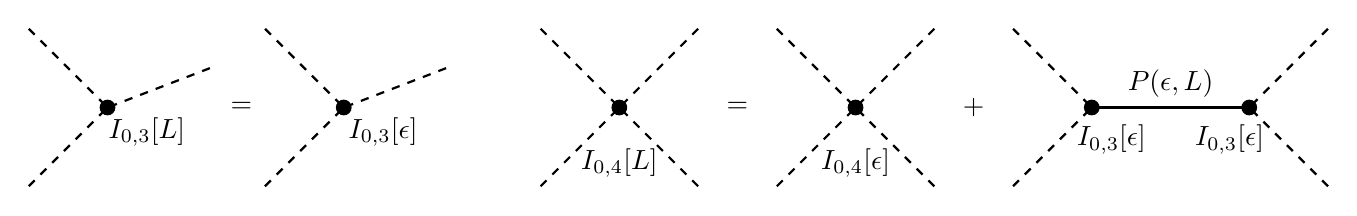
\begin{tikzpicture}
   \draw[thick, dashed] (-1.,-1.) -- (0,0);
   \draw[thick, dashed] (-1.,1.) -- (0,0);
   \draw[thick, dashed] (1.3,.5) -- (0,0);
   \fill [black] (0,0) circle (0.1) node[below, xshift=.5cm]{$I_{0,3}[\epsilon]$};
   \fill [black] (-1.3,0) circle (0.0) node[]{$=$};
   \draw[thick, dashed] (-1.-3.,-1.) -- (-3.,0);
   \draw[thick, dashed] (-1.-3.,1.) -- (-3.,0);
   \draw[thick, dashed] (1.3-3.,.5) -- (-3.,0);
   \fill [black] (-3.,0) circle (0.1) node[below, xshift=.5cm]{$I_{0,3}[L]$};


   \draw[thick, dashed] (5.5-3.,-1.) -- (6.5-3.,0);
   \draw[thick, dashed] (5.5-3.,1) -- (6.5-3.,0);
   \draw[thick, dashed] (7.5-3.,-1) -- (6.5-3.,0);
   \draw[thick, dashed] (7.5-3.,1) -- (6.5-3.,0);
   \fill [black] (6.5-3.,0) circle (0.1) node[below, xshift=.0cm, yshift=-.4cm]{$I_{0,4}[L]$};

   \draw[thick, dashed] (5.5,-1.) -- (6.5,0);
   \draw[thick, dashed] (5.5,1) -- (6.5,0);
   \draw[thick, dashed] (7.5,-1) -- (6.5,0);
   \draw[thick, dashed] (7.5,1) -- (6.5,0);
   \fill [black] (6.5,0) circle (0.1) node[below, xshift=.0cm, yshift=-.4cm]{$I_{0,4}[\epsilon]$};

   \fill [black] (5.,0) circle (0.0) node[]{$=$};
   \fill [black] (8,0) circle (0.0) node[]{$ + $};
   \fill [black] (9.5,0) circle (0.1) node[below, xshift=.25cm, yshift=-.1cm]{$I_{0,3}[\epsilon]$};
   \draw[thick, dashed] (8.5,-1.) -- (9.5,0);
   \draw[thick, dashed] (8.5,1) -- (9.5,0);
   \draw[thick] (9.5,0) -- (11.5,0) node[above, xshift=-1cm]{$P(\epsilon,L)$};
   \fill [black] (11.5,0) circle (0.1) node[below, xshift=-.25cm, yshift=-.1cm]{$I_{0,3}[\epsilon]$};
   \draw[thick, dashed] (12.5,-1) -- (11.5,0);
   \draw[thick, dashed] (12.5,1) -- (11.5,0);

 \end{tikzpicture}
\end{center}

The following ideas on taking limits of the above construction for $\epsilon \lra 0$ will be presented as a sketch rather than a more strict formulation. Note that this is due to time restrictions and the respectable overhead a strict treatment demands.

\begin{sketch}
  We consider $W(P(\epsilon,L), I(\epsilon))$ and $I(\phi) = \frac{1}{3!} \int_M \phi^3$. In particular we consider two graphs:

  \begin{center}
   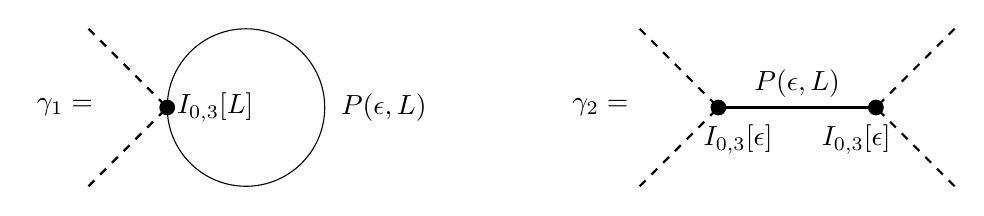
\begin{tikzpicture}
     \fill [black] (-1.3,0) circle (0.0) node[]{$\gamma_1 =$};
     \draw[thick, dashed] (-1.,-1.) -- (0,0);
     \draw[thick, dashed] (-1.,1.) -- (0,0);
     \draw (1.,0) circle (1cm) node[xshift=1.75cm]{$P(\epsilon,L)$};
     \fill [black] (0,0) circle (0.1) node[right, xshift=.0cm]{$I_{0,3}[L]$};

     \fill [black] (8-2.5,0) circle (0.0) node[]{$ \gamma_2 = $};
     \fill [black] (9.5-2.5,0) circle (0.1) node[below, xshift=.25cm, yshift=-.1cm]{$I_{0,3}[\epsilon]$};
     \draw[thick, dashed] (8.5-2.5,-1.) -- (9.5-2.5,0);
     \draw[thick, dashed] (8.5-2.5,1) -- (9.5-2.5,0);
     \draw[thick] (9.5-2.5,0) -- (11.5-2.5,0) node[above, xshift=-1cm]{$P(\epsilon,L)$};
     \fill [black] (11.5-2.5,0) circle (0.1) node[below, xshift=-.25cm, yshift=-.1cm]{$I_{0,3}[\epsilon]$};
     \draw[thick, dashed] (12.5-2.5,-1) -- (11.5-2.5,0);
     \draw[thick, dashed] (12.5-2.5,1) -- (11.5-2.5,0);

   \end{tikzpicture}
  \end{center}

  Now note that
  $$ w_{\gamma_1} (P(\epsilon,L), I(\epsilon))(a) = \int_{l\in[\epsilon,L]} \int_{x\in M} a^2(x) \ \kappa_l(x,x) \ d\vol_M dl$$
  Now if we take the limit $l \lra 0$ we obtain
  $$ \kappa_l(x,x) \simeq l^{-(\dim M)/2} + h.o.t. $$
  The problem is, that the integral over this term does not converge and thus
  $$ \lim_{\epsilon \lra 0} w_{\gamma_1} (P(\epsilon,L), I(\epsilon))(a) $$
  does not exist. For $\gamma_2$ we note that
  \begin{align*}
    w_{\gamma_2} (P(\epsilon,L), I(\epsilon))(a) &= \int_{l\in[\epsilon,L]} \int_{x,y\in M} a^2(x) \ \kappa_l(x,y) \ a^2(y) \ dx dy dl \\
    &= \left\langle a^2, \int_\epsilon^L e^{-lD} a^2 \ dl \right\rangle
  \end{align*}
  In this case the limit $\lim_{\epsilon \lra 0} w_{\gamma_2}$ does indeed exist!
\end{sketch}

Now this rough sketch can indeed be linked to a more general result:

\begin{fact}~
\begin{itemize}
  \item \textbf{graphs with loops do not have a limit} $\epsilon \lra 0$
  \item \textbf{graphs without loops (tree-level graphs) do have a limit} $\epsilon \lra 0$
\end{itemize}
\end{fact}

We will see in the subsequent material that and how we need to react to the infinities that arise when working with graphs that do contain loops.


\subsubsection{Interpretation of Feynman diagrams}
\label{subsubsec:feynman_intepretation}

The heat kernel can be interpreted as a form of transition propability such that we arrive at the following propability for a transition from $x$ to $y$:

$$ P(x,y) = \int_{l=0}^\infty e^{-lm^2} \int_{f\in X}  \exp\left( - \int_0^l ||df||^2 \right)$$
where $X = \{f \colon [0,l] \lra M | f(0) = x, f(l) = y \}$ is the space of paths from $x$ to $y$. Remember that we defined the energy of such a path as
$$ E(f) := - \int_0^l \langle df, df \rangle $$
Now we can collect this as
$$ P(x,y) = \int_0^\infty \kappa_l(x,y) \ dl $$
To make this integral well-defined, we also need the \emph{Wiener} measure, which we won't go into detail about:
$$ \kappa_f (x,y) = \int_X D_{Wiener} f $$
To consider a particular interaction and think about why it physically corresponds to Feynman graphs, we take

$$ S(\phi) = \int_M - \frac{1}{2} \phi D\phi + \frac{1}{3!} \phi^3 $$

note that this consideration is not necessarily well-defined and does contain quite some problems. Thus this discussion is more of a sketch. For $n$ particles we consider the expectation value

$$ \mathds{E}(x_1, x_2, ..., x_n) = \int_{\phi \in \Ci(M)} e^{S(\phi)/\hbar} \phi(x_1) ... \phi(x_n) $$

Now we associate to $n$ particles $n$ external edges:

$$ \mathds{E}(x_1, ..., x_n) = \sum_\gamma \frac{1}{|\Aut(\gamma)|} \hbar^{-\sigma(\gamma)} \int_{g \in Met_\gamma} \int_{f: \gamma \ra M} e^{-E(f)} $$
where $Met_\gamma$ stands for the space of metrics on the space of curves $\gamma$ and $f$ are those maps $\gamma \lra M$ that take the endpoints of the $n$ external edges of $\gamma$ to $x_1,...,x_n$. Also consider the inverse assignment
$$ f \colon \gamma \lra M, \quad \quad E(\gamma) \lmap (x_1,...,x_n) $$

\begin{definition}[Local action functional]
  A functional $I \in \OO(\Ci(M))$ that can be written as $I = \sum_k I_k$ where $I_k$ is homogenous of degree $k$ in the variable $a \in \Ci(M)$, that is
  $$ I_k(\lambda a) = \lambda^k I_k(a) $$
  and such that the $I_k$ can be written as
  $$ I_k (a) = \sum_{j=1}^{S} \int_M D_{1,j} (a) ... D_{k,j} (a) $$
  where $D_{i,j}$ are differential operators on $M$ is called a \textbf{local action functional}.
\end{definition}

We will subsequently denote by $\OO_{loc}(\Ci(M))$ the \textbf{subspace of local action functionals}. This definition extends to the formal power series in $\hbar$ that is $I \in \OO(\Ci(M))\llbracket \hbar \rrbracket$ as follows:
$$ I = \sum_{i,k} \hbar^i I_{i,k} $$
where the $I_{i,k}$ need to be in $\OO_{loc}(\Ci(M))$. We further define
$$ \OO^+_{loc}(\Ci(M))\llbracket \hbar \rrbracket \subset \OO_{loc}(\Ci(M))\llbracket \hbar \rrbracket $$
the subspae of local functionals which are at least cubic modulo $\hbar$. Finally we are prepared to define scalar QFTs:

\begin{definition}[Perturbative scalar quantum field theories]
\label{def:PSQFTs}
  A \textbf{perturbative scalar quantum field theory} is given by a set of effective interactions
  $$ I[L] \in \OO^+_{loc}(\Ci(M))\llbracket \hbar \rrbracket \quad \forall L \in [0, \infty] $$
  (plus a kinetic action $- \frac{1}{2} \langle \phi, (D + m^2) \phi \rangle$ for $\phi \in \Ci(M)$) such that
  \begin{enumerate}
    \item $I[L] = W(P(\epsilon, L), I[\epsilon]) \quad \forall \epsilon,L \in (0,\infty)$

    \item Let
    $$ I[L] = \sum_{i,k} \hbar^i I_{i,k}[L] $$
    For each $i,k$ we require a small-$L$ asymptotic expansion
    $$ I_{i,k}[L] \simeq \sum_{r \in \ZZ} g_r(L) \Phi_r $$
    where $g_r(L) \in \Ci((0,\infty)_L)$ and $\Phi_r \in \OO_{loc}(\Ci(M))$. Small-$L$ asymptotic expansion means that there exists a non-decreasing sequence
    $$ d_R \in \ZZ, \quad d_R \lra \infty, \quad R\lra \infty $$
    such that for all $R$
    $$ \lim_{L \lra 0} L^{-d_R} \left( I_{i,k}[L](a) - \sum_{r=0}^R g_r(L) \Phi_r(a) \right) = 0 $$
    for all $a \in \Ci(M)$.
  \end{enumerate}
  We will denote by $\mathcal{Z}^{(a)}$ the set of perturbative quantum field theories and by $\mathcal{Z}^{(n)}$ the set of such theories defined modulo $\hbar^{n+1}$, that is ignoring terms in $\hbar$ of order higher than $n$. Further we denote
  $$ \mathcal{Z}^{(\infty)} = \lim_{\longleftarrow} \mathcal{Z}^{(n)} $$
\end{definition}

\subsection{The structure of scalar perturbative QFTs}

We now have a definition of quantum field theory and we might ask how we can connect it to a classical definition of quantum field theory without any effective interactions. This connection can be formulated in the following theorem:

\begin{theo}
  $\mathcal{Z}^{(n+1)}$ is a principal bundle over $\mathcal{Z}^{(n)}$ with structure group the abelian group $\OO_{loc}(\Ci(M))$ (local action functionals on $M$). In particular, $\mathcal{Z}^{(0)}$ is canonically isomorphic to the space $\OO^+_{loc}(\Ci(M))$
\end{theo}

\begin{theo}
  If we fix a \emph{normalisation scheme} (which we will define and explain later), we can find a section for each torsor $\mathcal{Z}^{(n+1)} \lra \mathcal{Z}^{(n)}$ and consequently a bijection between the set of perturbative quantum fields theories and the set of local action functionals $I \in \OO^+_{loc}(\Ci(M))\llbracket \hbar \rrbracket$.
\end{theo}

While we might not find the time to discuss the proofs of the two above theorems, their statements are the most important points. The first one provides convenient and interesting structure, mainly telling us that once we restrict to the classical setting, we recover a classical action functional, hence providing a canonical transition from quantum to classical. The second theorem provides a direct link between local action functionals and perturbative QFTs, thus enabling the transition shown in the first.\\

We now discuss a \textit{strategy} to work with both of these statements: First fix $I \in \OO^+_{loc}(\Ci(M))\llbracket \hbar \rrbracket$. We want to build the effective interaction $I[L]$ satisfying the properties of its definition. So first of all we want to construct counterterms $I^{CT}(\epsilon)$ such that
$$ \lim_{\epsilon \lra 0} W\left(P(\epsilon,L), I-I^{CT}(\epsilon)\right)$$
exists and in particular defines $I[L]$. Conversely given $\{I[L]\}$ we construct $I$ as a renormalised limit, subtracting the suitable counterterms. To this end, we define some new helpful notions:

\begin{definition}[Periods]
  Into the classical sequence $\NN \subset \ZZ \subset \QQ \subset \ABF \subset \RR$ we want to insert $\ABF \subset \PP \subset \RR$ where $\PP$ forms a ring contained in transcendental and algebraic numbers. A \textbf{period} is a complex number whose real and imaginary part are values of absolutely converging integrals of rational functions with rational coefficients over domains in $\RR^n$ given by polynomial inequalities with rational coefficients.
  %TODO graph?
\end{definition}

\begin{example}
  Two numbers included in $\PP$ and clearly not included in $\QQ$ are:
  \begin{align*}
    \sqrt{2} &= \int_{2x^2 \leq 1} dx \\
    \pi &= \iint_{x^2+y^2\leq 1} dx dy = 2 \int_{-1}^{+1} \sqrt{1-x^2} dx
  \end{align*}
\end{example}

Now let $t \in (0, \infty)$ be a real parameter. Formally we might write a "period depending smoothly on $t$" as
$$ \alpha(t) = \int_{\gamma(t)} \omega(t) $$
where we allow $\gamma(t)$ and $\omega(t)$ to depend smoothly on $t$. But of course we further need to require that $\alpha(t)$ is a period, thus $\in \PP$, for every rational number $t \in \QQ \cap (0,\infty)$. Collecting these requirements leads us to a definition from \emph{algebraic geometry}:

\begin{definition}[Periods in Algebraic Geometry]
  We call \textbf{rational periods} those functions in $\Ci((0,\infty))$ which are of this form and denote by $P_\QQ((0,\infty))$ the set of rational periods.
\end{definition}

\begin{definition}
  We define $\mathcal{P}((0,\infty))$ to be the real vector space spanned by the space of rational periods:
  $$ \mathcal{P}((0,\infty)) = P_\QQ((0,\infty)) \otimes \RR \subset \Ci((0,\infty)) $$
  By an abuse of notation, we call elements of $\mathcal{P}((0,\infty))$ \textbf{periods}.
\end{definition}

Now we still investigate $w_\gamma(P(\epsilon,L), I(\epsilon))(a)$ in the limit $\epsilon \lra 0$. We interpret $w_\gamma$ as a function of $\epsilon,L,a$, thus in
$$ \OO(\Ci(M), \Ci((0,\infty)_\epsilon)) \otimes \Ci((0,\infty)_L) $$
In particular, if we fix $\epsilon$, we have
$$ w_\gamma \in \OO(\Ci(M), \Ci((0,\infty)_L)) $$
This leads us to the following theorem:

\begin{theo}
  Let $I \in \OO_{loc}(\Ci(M))\llbracket \hbar \rrbracket$ be a local action functional and let $\gamma$ be a connected stable graph. Then there exists a small-$\epsilon$ asymptotic expansion
  $$ w_\gamma (P(\epsilon,L), I[\epsilon]) \simeq \sum_{i=0}^{\infty} g_i(\epsilon) \psi_i $$
  where $g_i \in \mathcal{P}((0,\infty)_\epsilon)$ are periods and $\psi_i \in \OO(\Ci(M), \Ci((0,\infty)_L))$ such that
  \begin{enumerate}
    \item $$ \lim_{\epsilon\lra 0} L^{-d_R} \left(w_\gamma - \sum_{r=0}^R g_r(\epsilon) \psi_r \right) = 0 \quad \forall a \in \Ci(M) $$

    \item the $g_i(\epsilon)$ have finite order poles at $0$, i.e. for $\forall i \ \exists k$ such that
    $$ \lim_{\epsilon\lra 0} \epsilon^k g_i(\epsilon) = 0 $$

    \item the $\psi_i$ have a small-$L$ asymptotic expansion of the form
    $$ \psi_i \simeq \sum_{j=0}^{\infty} f_{i,j} (L) \psi_{i,j} $$
    where $\psi_{i,j} \in \OO_{loc}(\Ci(M))$ and $f_{i,j} \in \Ci((0,\infty)_L)$.
  \end{enumerate}
\end{theo}

Sadly we won't have the time to prove the above theorem since it is rather lengthy and technical. Thus we go on with the following definition:

\begin{definition}
  Define $\mathcal{P}((0,\infty))_{\geq 0} \subseteq \mathcal{P}((0,\infty))$ to be the subspace of functions of $\epsilon$ that are periods and which admit a limit as $\epsilon \lra 0$.
\end{definition}

Using this definition we can finally expand upon the previously mentioned \emph{renormalisation schemes}:

\begin{definition}{Renormalisation Schemes}
  A choice of a subspace
  $$ \mathcal{P}((0,\infty))_{< 0} \subset \mathcal{P}((0,\infty))  $$
  complementary to $\mathcal{P}((0,\infty))_{\geq 0}$ is called a \textbf{renormalisation scheme}. Hence a renormalisation scheme provides a direct sum decomposition
  $$ \mathcal{P}((0,\infty))_{\geq 0}((0,\infty)) = \mathcal{P}((0,\infty))_{\geq 0}((0,\infty))_{\geq 0} \oplus \mathcal{P}((0,\infty))_{< 0} $$
\end{definition}

Introducing further notation using the decomposition at hand we define

\begin{definition}[Singular Parts]
  Given a period $f \in \mathcal{P}((0,\infty))$ define its \textbf{singular part} to be the projection $\sing(f)$ of $f$ onto $\mathcal{P}((0,\infty))_{< 0}$.
\end{definition}

\textbf{From now on, we fix a renormalisation scheme.} From the previous theorem, take
$$ w_\gamma (P(\epsilon,L), I[\epsilon]) \simeq \sum_{i=0}^{\infty} g_i(\epsilon) \psi_i $$
Now there exists an $N$ such that $\forall n > N$ the $g_n(\epsilon)$ admits a limit $\epsilon \lra 0$. As an \textbf{exercise} you can prove this claim. Now define
$$ \psi_N := \sum_{i=0}^N g_i(\epsilon) \psi_i $$
and note that
$$ \sing_\epsilon (w_\gamma(P(\epsilon,L), I[\epsilon])) := \sing( \psi_N(\epsilon)) = \sum_{i=0}^N \sing_\epsilon(g_i(\epsilon)) \psi_i $$
We can collect these results and definitions into a theorem:

\begin{theo}
  Let $I \in \OO_{loc}(\Ci(M)) \llbracket \hbar \rrbracket$ be a local action functional and let $\gamma$ be a connected stable graph. Then
  $$ \sing_\epsilon(w_\gamma(P(\epsilon,L), I[\epsilon])) = \sum_i f_i(\epsilon) \psi_i  $$
  where $f_i(\epsilon) \in \mathcal{P}((0,\infty))_{\geq 0}$ are singular periods (periods equivalent to their singular part) and the $\psi_i$ have a small-$L$ asymptotic expansions of the form
  $$ \phi_i \simeq \sum_{i = 0}^\infty f_{i,j} \psi_{i,j} $$
  where $\psi_{i,j} \in \OO_{loc}(\Ci(M))$ and $f_{i,j} \in \Ci((0,\infty)_L)$. Furthermore the limit
  $$ \lim_{\epsilon \lra 0} \left( w_\gamma (P(\epsilon,L), I[\epsilon]) - \sing_\epsilon(w_\gamma (P(\epsilon,L), I[\epsilon])) \right) $$
  exists in $\OO_{loc}(\Ci(M), \Ci((0,\infty)_L))$.
\end{theo}

\begin{theo}
  There exists a unique series of local counterterms
  $$ I_{i,k}^{CT}(\epsilon) \in \OO_{loc}(\Ci(M)) \otimes \mathcal{P}((0,\infty))_{<0} $$
  for any $i,k$ with $I_{i,k}^{CT}$ homogenous of degree $k$ as a function of $a \in \Ci(M)$ and such that for all $L \in (0,\infty)$ the limit
  $$ \lim_{\epsilon \lra 0} W(P(\epsilon, L), I - \sum_{i,k} \hbar^i I_{i,k}^{CT}(\epsilon)) $$
  exists.
\begin{proof}
  First note that
  \begin{align*}
    W(P,I) &= \sum_{i,k} \hbar^i W_{i,k}(P,I) \\
    W_{i,k}(P,I) &= \sum_{\gamma \in \Gamma_{i,k}} w_\gamma (P(\epsilon, L), I[\epsilon])
  \end{align*}
  where $\Gamma_{i,k}$ is the set of all stable graphs of genus $i$ with $k$ external edges. Now for $i = 0$ the term
  $$ \lim_{\epsilon \lra 0} w_\gamma (P(\epsilon, L), I[\epsilon])$$
  converges. Now for $i\neq 0$ we denote
  $$ (i,j) < (k,l) \quad \Leftrightarrow \quad i<k \ or \ (i=k \ and \ j<l) $$
  Thus define
  $$ I_{1,1}^{CT}(\epsilon, L) = \sing_\epsilon(W_{1,1}(P(\epsilon, L), I[\epsilon])) $$
  To show that this is indeed a fitting counterterm, we calculate
  \begin{align*}
    W_{1,1}(P(\epsilon,L), I[\epsilon] - \hbar I_{1,1}^{CT}(\epsilon,L)) &= W_{1,1}(P(\epsilon,L), I[\epsilon]) - I_{1,1}^{CT}(\epsilon,L)\\
    \Rightarrow \quad W_{1,1}(P(\epsilon,L), \hbar I_{1,1}^{CT}(\epsilon,L)) &= I_{1,1}^{CT}
  \end{align*}
  Thus taking the limit we obtain
  \begin{align*}
    &\lim_{\epsilon \lra 0} W_{1,1}(P(\epsilon,L), I[\epsilon] - \hbar I_{1,1}^{CT}(\epsilon,L)) \\
    = &\lim_{\epsilon \lra 0} \left( \Reg_\epsilon(W_{1,1}(P(\epsilon,L))) + \sing_\epsilon(W_{1,1}(P(\epsilon,L))) - \sing_\epsilon(W_{1,1}(P(\epsilon,L))) \right)
  \end{align*}
  and thus the limit exists. Now we want to show that $I_{1,1}^{CT}$ is local. To this end note that
  \begin{align*}
    \dd{}{L} W_{1,1}(P(\epsilon,L))
    %TODO graphs?
  \end{align*}
  Since $K_L$ is smooth the singular point of the derivative is zero. Further the singular point of $W_{1,1}$ does not depend on $L$ which implies
  $$ I_{1,1}^{CT}(\epsilon, L) = I_{1,1}^{CT}(\epsilon) $$
  Now recall that
  $$ \sing_\epsilon w_\gamma = \sum_i f_i(\epsilon) \phi_i $$
  where the $\phi_i$ have a small-$L$ asymptotic expansion. Thus $\sing_\epsilon w_\gamma$ is local. Having established the base case, we now use induction to conclude the proof:\\
  Suppose we have constructed $I_{j,l}^{CT}(\epsilon)$ for all $(j,l)<(i,k)$ such that they satisfy our theorem. For convenience we define
  \begin{align*}
    W_{<(i,k)} (P,I) &= \sum_{(j,l)<(i,k)} \hbar^j W_{j,l}(P,I)\\
    &= \sum_{\gamma \in \Gamma_{<(i,k)}} \frac{\hbar^{g(\gamma)}}{|\Aut(\gamma)|} w_\gamma (P,I)
  \end{align*}
  Now we define the counterterms as
  $$ I_{i,k}^{CT}(\epsilon, L) = \sing_\epsilon W_{i,k}\left(P(\epsilon,L), I - \sum_{(j,l)<(i,k)}\hbar^j I_{j,l}^{CT}(\epsilon)\right) $$
  Thus we again investigate the limit of
  \begin{align*}
    &W_{i,k}\left( P(\epsilon,L), I - \sum_{(j,l)<(i,k)}\hbar^j I_{j,l}^{CT}(\epsilon) - \hbar^i I_{i,k}^{CT}(\epsilon, L) \right)\\
    = \quad &W_{i,k}\left( P(\epsilon,L), I - \sum_{(j,l)<(i,k)}\hbar^j I_{j,l}^{CT}(\epsilon) \right) - I_{i,k}^{CT}(\epsilon, L)
  \end{align*}
  We see that the limit for $\epsilon \lra 0$ exists. Now all we need to show is that $I_{i,k}^{CT}(\epsilon,L)$ is local which is done as before by showing that it is independent on $L$.
\end{proof}
\end{theo}

Now let $I \in \OO^+(\Ci(M))\llbracket\hbar\rrbracket$ be a local action functional. We define
$$ I[L] := \lim_{\epsilon \lra 0} \left( W(P(\epsilon,L), I - I^{CT}(\epsilon)) \right) =: W^R(P(0,L), I) $$
where $I \simeq I(\epsilon \ra 0) $.

\begin{ex}
  Prove that $I[L]$ satisfies the \eqref{eq:RGE_length} and the small-$L$ asymptotic expansion of the definition of a scalar PQFT.
\end{ex}

Conversely, let $\{I[L]\}$ be a collection of effective actions defining a theory. Now for
$$ I = \sum_{i,k} \hbar^i I_{i,k} $$
we want to construct the terms $I_{i,k}$. For $I_{0,0}$ just take the limit $\lim_{\epsilon \ra 0} W(P(\epsilon,L), I[L])$. Now let us suppose we have constructed $I_{r,s}$ for $(r,s)<(i,k)$ such that
$$ W^R_{a,b}\left(P(0,L), \sum_{(r,s)<(i,k)} \hbar^k I_{r,s}\right) = I_{a,b}(L)$$
for all $(a,b) < (i,k)$. Now
$$I_{i,k} = I_{i,k}[L] - W^R_{i,k}\left(P(0,L), \sum_{(r,s)<(i,k)} \hbar^r I_{r,s} \right)$$
Thus recall
$$ W^R(P(0,L), I) = \sum_{i,k} \hbar^i W_{i,k}^R (P(0,L), I) $$

\begin{ex}
  Show that this quantity does not depend on $L$ (use \eqref{eq:RGE_length}) and is local (use the locality of $\{I[L]\}$).
\end{ex}

Thus we have established a bijection between theories and local power series in $\hbar$
\begin{align}
  \ZZ^{(\infty)} &\underset{RS}{\longleftrightarrow} \OO^+_{loc}(\Ci(M))\llbracket \hbar \rrbracket \\
  \ZZ^{(n)} &\underset{RS}{\longleftrightarrow} \OO^+_{loc}(\Ci(M))\llbracket \hbar \rrbracket / \hbar^{n+1}
\end{align}


\subsection{Principal Bundle}
\subsection{Renormalisability}

\textbf{Problem:} The space of theories is an infinite-dimensional manifold. Physically, to specify a particular theory we would need an infinite number of experiments.\\

Thus we want to consider a finite subset of these theories, namely renormalisable theories. \textbf{Classically} a theory is renormalisable, if it has a finite number of counterterms. But we saw that the number of counterterms depends on the choice of renormalisation scheme.

\begin{axiom}
  A theory $\{S^{eff}[\Lambda]$ is renormalisable if $S^{eff}[\Lambda]$ does not grow too fast when $\Lambda \lra \infty$, measured in the "right" units appropriate to the energy scale.
\end{axiom}


\textbf{Aside:} If $M = \RR^n$, it is not compact, but we can define a scalar PQFT in (more or less) the same way and get similar results. Define
$$ R_l \colon \Ci(\RR^n) \lra \Ci(\RR^n), \quad \quad \phi(x) \lmap l^{1-n/2} \phi(l^{-1} x) $$
and additionally the map
$$ RG_l (S^{eff}[\Lambda]) (\phi) = S^{eff}[l^{-2} \Lambda](R_l(\phi)) $$
This leads us to the following result:

\begin{lem}
  $RG_l$ is a flow on the space of theories. If $ \{S^{eff}[\Lambda]\}$ satisfies the \eqref{eq:RGE}, then so does $\{RG_l(S^{eff}[\Lambda])\}$. We call $RG_l$ the \textbf{local renormalisation group flow}.
\end{lem}


\begin{definition}
  A theory is \textbf{renormalisable} if $RG_l(S^{eff}[\Lambda])$ grows, in terms of $\Lambda$, at most logarithmically as $l \lra 0$. Suppose that $S$ is translation invariant. We say that $S$ is of dimension $k$ if
  $$ S(R_l(\phi)) = l^k S(\phi) $$
\end{definition}

\begin{example}~
  \begin{itemize}
    \item $\int_{\RR^4} \phi D \phi, \ \int \phi^4$ are of $\dim 0$.
    \item $\int_{\RR^4} \phi^2$ is of $\dim 2$.
  \end{itemize}
\end{example}

\begin{theo}
  Let $\mathfrak{R}^{(k)}(\RR^n)$ be the space of renormalisable scalar field theories of $\RR^n$ invariant under translation defined modulo $\hbar^{n+1}$. Then
  $$  \mathfrak{R}^{(k+1)}(\RR^n) \lra \mathfrak{R}^{(k)}(\RR^n)$$
  is a torsor for the vector space of local action functionals $S(\phi)$ which are a sum of terms of non-negative dimensions. Furthermore $\mathfrak{R}^{(0)}(\RR^n)$ is canonically isomorphic to the space of local action functionals of the form
  $$ S(\phi) = \frac{1}{2} \int_{\RR^n} \phi D \phi + I $$
  where the $I$ are cubic or higher terms of non-negative dimensions.
\end{theo}

\begin{corollary}
  On $\RR^4$ renormalisable scalar field theories invariant under $SO(4) \times RR^4$ and $\phi \lmap -\phi$ are in bijection with Lagrangians of the form
  $$ \LL (\phi) = a \phi D \phi + b \phi^4 + c \phi^2 $$
  for $a,b,c \in \RR\llbracket\hbar \rrbracket$ and such that $a = - \frac{1}{2}$ modulo $\hbar$ and $c = 0$ modulo $\hbar$.
\end{corollary}




\newpage
